\label{pierwsze_uruchomienie}
\begin{wrapfigure}{R}{0.5\textwidth}
                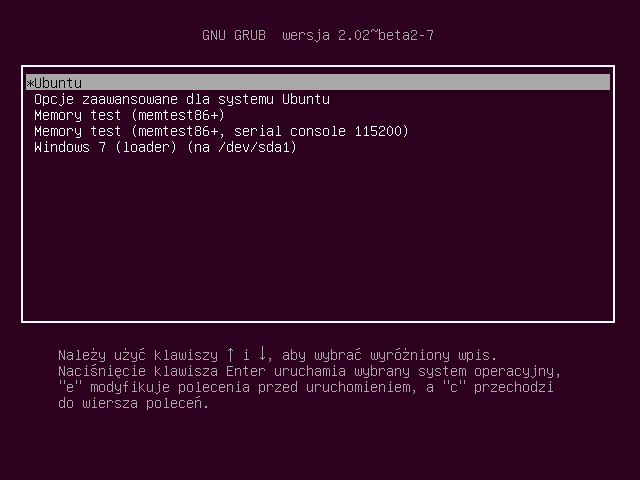
\includegraphics[width=\linewidth]{images/pierwsze_uruchomienie_grub.png}
\end{wrapfigure}

Po zainstalowaniu systemu Ubuntu twój komputer został zresetowany, zostałeś też poproszony o usunięcie nośnika instalacyjnego (pendrive, płyta DVD) z napędu. Jeżeli to wykonałeś to przy ponownym uruchomieniu komputera powinieneś zobaczyć ekran bardzo podobny do tego. Jest to GRUB (\textcolor{ubuntu_orange}{Grand Unified Bootloader}), program rozruchowy zajmujący uruchomieniem systemu operacyjnego. Korzystając z GRUBA możesz wybrać, który system operacyjny ma zostać uruchomiony. Korzystając z klawiszy kursora na klawiaturze podświetl odpowiednią opcję i wciśnij \keys{\returnwin}.

Jeżeli Ubuntu to jedyny system operacyjny zainstalowany na twoim komputerze to menu GRUBa nie wyświetli się. Zamiast niego Przez około sekundę widoczny będzie ciemnofioletowy ekran a następnie zostanie uruchomiony system Ubuntu. Aby w takiej sytuacji wejść do menu GRUBa wciśnij klawisz \keys{Shift} kiedy fioletowy ekran jest widoczny.

\begin{itemize}
\item \textcolor{ubuntu_orange}{Opcje zaawansowane dla systemu Ubuntu} to zestaw dodatkowych programów naprawczych i diagnostycznych dla systemu Ubuntu. Zostały one szerze opisane w rozdziale \ref{rozwiązywanie problemów}: ,,Rozwiązywanie Problemów''.
\item \textcolor{ubuntu_orange}{Memorytest} to program służący do testowania pamięci operacyjnej komputera (RAM).
\item \textcolor{ubuntu_orange}{Windows 7 Loader} uruchomi system operacyjny Windows 7.
\end{itemize}

Ilość pozycji w menu będzie się różnić w zależności od tego ile i jakie systemy operacyjne masz zainstalowane na swoim komputerze.

\begin{flushright}
Wybierz \textcolor{ubuntu_orange}{Ubuntu}, wciśnij klawisz \keys{\returnwin} aby uruchomić Ubuntu.
\end{flushright}
\clearpage
